\documentclass[12pt,fleqn]{beamer}
\usepackage{xcolor}
\usetheme{AnnArbor}
\usecolortheme{beaver}
\usepackage{setspace}
\usepackage{cancel}
\usepackage{tcolorbox}
\addtobeamertemplate{frametitle}{}{\vspace{-0.4em}} 
\newcommand{\question}[1]{\textcolor{blue}{#1}}
\setbeamertemplate{itemize items}[ball]
\makeatother
\title{KIX1001 Tutorial 1}
\author[Hong Vin]{}
\date{October 29, 2021}
\begin{document}

%%% Question 1 %%%
\begin{frame}[t]
\frametitle{Question 1}

\question{Find $y'$ for $(x-y)^{2}=x+y-1$ by using implicit differentiation.}

\scalebox{0.8}{\begin{minipage}{1.20\textwidth}
\[
\begin{align*}
\mathcal{D} (x-y)^{2} & =\mathcal{D} (x+y-1)\\\pause
\mathcal{D} (x-y)^{2} & =\mathcal{D} (x)+\mathcal{D} (y)-\mathcal{D} (1)\\\pause
2(x-y)\mathcal{D} (x-y) & =1+y'\\\pause
2(x-y)(1-y') & =1+y'\\\pause
2(x-y)-2(x-y)y' & =1+y'\\\pause
-2(x-y)y'-y' & =1-2(x-y)\\\pause 
y'[-2(x-y)-1] & =1-2(x-y)\\\pause 
y' & =\frac{1-2(x-y)}{-2(x-y)-1}\\\pause 
y' & =\boldsymbol{\frac{2y-2x+1}{2y-2x-1}}
\end{align*}
\]
\end{minipage}}
\end{frame}

%%% Question 2 %%%
\begin{frame}[t]
\frametitle{Question 2}

\question{Implicit differentiation to find an equation of the tangent line to the curve $5x^{2} +10xy^{2} +5y=20$ at point $(2,2)$.}

\scalebox{0.8}{\begin{minipage}{1.20\textwidth}
\[
\begin{align*}
\mathcal{D} (5x^{2} +10xy^{2} +5y) & =\mathcal{D} (20)\\\pause 
10x+10x(2y\cdot y')+y^{2} \cdot 10+5y' & =0\\\pause 
10x+20xy\cdot y'+10y^{2} +5y' & =0\\\pause 
(20xy+5)y' & =-10y^{2} -10x\\\pause 
y' & =\frac{-10y^{2} -10x}{20xy+5}
\end{align*}
\]

\uncover<6-9>{At point $(2,2)$, $y'=\frac{-10(2)^{2} -10(2)}{20(2)(2) +5} =-\frac{12}{17}$}

\vspace{0.5em}
\uncover<7-9>{Knowing $y=mx+c$, }

\vspace{0.5em}
\uncover<8-9>{$2=-\frac{12}{17} (2)+c\rightarrow c=\frac{58}{17}$}

\vspace{0.5em}
\uncover<9>{$\therefore \text{Tangent Line: }\boldsymbol{y=-\frac{12}{17} x+\frac{58}{17}}$}

\end{minipage}}
\end{frame}

%%% Question 3 %%%
\begin{frame}[t]
\frametitle{Question 3}

\question{$y\cos x=1+\sin(xy)$. Find $\frac{dy}{dx}$ by implicit differentiation.}

\[
\begin{align*}
y\cos x & =1+\sin (xy)\\\pause
y(-\sin x)+(\cos x)y' & =\cos (xy)\cdot (xy'+y)\\\pause
-y\sin x+y'\cos x & =(xy'+y)\cos (xy)\\\pause
y' & =\boldsymbol{\frac{y\cos (xy)+y\sin x}{\cos x-x\cos xy}}
\end{align*}
\]
\end{frame}

%%% Question 4 %%%
\begin{frame}[t]
\frametitle{Question 4}

\question{Find $\frac{dy}{dx}$ by implicit differentiation $4\cos x\sin y=1$.}

\[
\begin{align*}
4\cos x\sin y & =1\\\pause
(4\cos x)\cdot (\cos y)\cdot y'+(\sin y)\cdot (-4\sin x) & =0\\\pause
y' & =\frac{4\sin x\sin y}{4\cos x\cos y}\\\pause
 & =\boldsymbol{\tan x\tan y}
\end{align*}
\]
\end{frame}

%%% Question 5 %%%
\begin{frame}[t]
\frametitle{Question 5}

\question{An open box is to be made from cutting a square from each corner of a 12 in by 12 in piece of metal and then folding up the sides. What size square should be cut from each corner to produce a box of maximum volume?}

\scalebox{0.6}{\begin{minipage}{1.60\textwidth}
\begin{columns}
\column{0.4\linewidth}
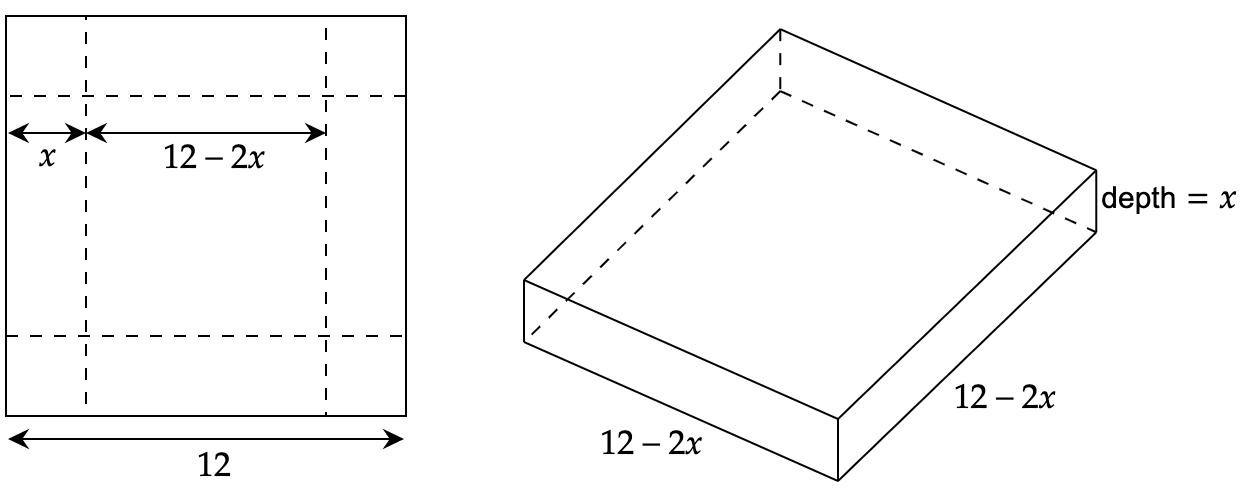
\includegraphics[width=\textwidth]{images/t2.1.png}

\uncover<2-15>{The volume is to be maximized, 
\vspace{0.5em}
\begin{align*}
V&=lwh=x(12-2x)(12-2x)\\
&=4x^{3} -48x^{2} +144x
\end{align*}}

\begin{align*}
\uncover<3-15>{V(x) & =4x^{3} -48x^{2} +144x\\}
\uncover<4-15>{V'(x) & =12x^{2} -96x+144}
\end{align*}


\column{0.55\linewidth}

\uncover<5-15>{The critical point can be calculate such that, $\displaystyle V'( x) =0$.}

\begin{align*}
\uncover<6-15>{0 & =12x^{2} -96x+144\\}
\uncover<7-15>{0 & =12(x^{2} -8x+12)\\}
\uncover<8-15>{0 & =12(x-2)(x-6)\\}
\uncover<9-15>{\therefore x & =2,6}
\end{align*}

\uncover<10-15>{When $x=2$, $V( 2) =128$. \quad When $x=6$, $V(6) =0$.}

\vspace{0.5em}
\uncover<11-15>{Thus, when $x=2$, the maximum volume is 128 in$^{3}$. }
\vspace{0.5em}
\uncover<12-15>{To prove that, using second derivation $V''(x) =24x-96$.}

\vspace{0.5em}
\uncover<13-15>{When $x=2$, $V''(2) < 0$ (Maximum Volume)}

\vspace{0.5em}
\uncover<14-15>{When $x=6$, $V''(6) > 0$ (Minimum Volume)}

\vspace{0.5em}
\uncover<15>{Thus, $\mathbf{x=2}$.}

\end{columns}
\end{minipage}}

\end{frame}

%%% Question 6 %%%
\begin{frame}[t]
\frametitle{Question 6}

\question{We are going to fence in a rectangular field. If we look at the field from above the cost of the vertical sides are RM 10/ft, the cost of the bottom is RM2/ft and the cost of the top is RM 7 /ft. If we have RM 700 determind the dimensions of the field that will maximize the enclosed area.}

\scalebox{0.6}{\begin{minipage}{1.60\textwidth}
\begin{columns}
\column{0.4\linewidth}

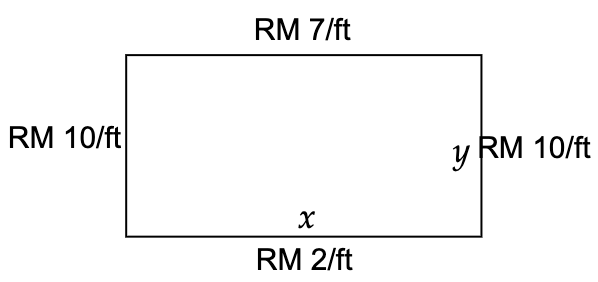
\includegraphics[width=\textwidth]{images/t2.2.png}

\uncover<2-12>{We have RM 700, therefore 
$700=10y+2x+10y+7x=20y+9x$.}

\vspace{0.5em}
\uncover<3-12>{In terms of $y$, $y=35-\frac{9}{20} x$.}

\vspace{0.5em}

\uncover<4-12>{Since $A=xy$, plugging in yields 

$A( x) =x\left(35-\frac{9}{20}x\right)$.}

\column{0.25\linewidth}

\uncover<5-12>{The critical point can be calculate such that, $A'(x) =0$.}

\begin{align*}
\uncover<6-12>{A'(x) & =35-\frac{9}{10} (x)\\}
\uncover<7-12>{0 & =35-\frac{9}{10} (x)\\}
\uncover<8-12>{\therefore x & =\frac{350}{9}}
\end{align*}


\uncover<9-12>{The second derivation,

$A''(x)=-\frac{9}{10}$}

\column{0.35\linewidth}
\uncover<10-12>{This means that the second derivative always negative and so $\displaystyle A( x)$ will always be concave down and so the single critical point. Therefore the value obtained in $\displaystyle A'( x)$ must be the value that yield maximum area.}

\vspace{0.5em}
\uncover<11-12>{Substituting $x=\frac{350}{9}$ into the equation of $y$, 

\vspace{0.5em}
$y=35-\frac{9}{20}\left(\frac{350}{9}\right) =\frac{35}{2}$}

\vspace{0.5em}
\uncover<12>{Thus, the final dimension is, $\mathbf{x=\frac{350}{9} ,y=\frac{35}{2}}$.}

\end{columns}
\end{minipage}}
\end{frame}


\end{document} 